\documentclass[a4paper,14pt]{extreport}

\usepackage{mathtools}
\usepackage{graphicx}
\usepackage{./diss_style}

% NOTE: Check for � always! They seem to creep up.

% Bibliography style
\usepackage[
style=gost-numeric, %or just numeric
backend=biber,
%sorting=ynt,
language=auto
]{biblatex}

\addbibresource{citations.bib}

% Оформление глав, разделов и т.д.
\makeatletter

% Values

\title{Разработка алгоритмов машинного обучения для построения моделей с переключением состояний}
\authorlast{Макаревич}
\authorfirst{Анатолий Сергеевич}
\author{\@authorlast \@authorfirst}

\mentor{Малюгин Владимир Ильич}
\mentorjob{доцент, кандидат физико-математических наук, кафедра ММАД}
\faculty{Факультет Прикладной Математики и Информатики}
\subfaculty{Кафедра Математического Моделирования и Анализа Данных}
\specialty{ПКАД (Прикладной Компьютерный Анализ Данных)}

\begin{document}

% Create title page
\maketitle

% ABSTRACT

% \begin{abstract}
% 	Аннотация на русском.
% \end{abstract}

% \selectlanguage{english}

% \begin{abstract}
% 	Abstract in English.
% \end{abstract}

\selectlanguage{russian}

% Общая характеристика работы
% «Общая характеристика работы» содержит:
% перечень ключевых слов; 
% цель, задачи, объект и предмет исследования;
% формулировку полученных результатов и их новизну;
% сведения о структуре магистерской диссертации. 
% Перечень ключевых слов характеризует основное содержание магистерской диссертации и включает 10-15 слов в именител/ьном падеже, написанных через запятую в строку прописными буквами. 

\fakechapter{Реферат}

Работа: N стр., N табл., N рис., N источников, N приложений

\MakeUppercase{временные ряды, модели с переключением состояний, анализ поворотных точек экономических циклов}

Объекты исследования -- математические модели временных рядов, использующие переключение состояния; индикаторы экономики Республики Беларусь.

Цель работы -- исследование свойств моделей с переключением состояния (а также подклассы MS-VARX, IS-VARX) и их применение к задачам эконометрического моделирования на примере определения поворотных точек бизнес-цикла ВВП Республики Беларусь.

Методы исследования -- компьютерное моделирование временных рядов (индикаторы экономики Республики Беларусь и сгенерированные ряды). Используются как классические, так и байесовские статистические подходы.

В результате исследования получены новые модели для годовых темпов роста ВВП РБ, подтверждение опережающего характера индикатора экономических настроений (ИЭН), а также новые подходы к оценке параметров более общих RS-моделей.


% ОГЛАВЛЕНИЕ

\clearpage
\renewcommand{\contentsname}{Содержание}
\tableofcontents


% Перечень условных обозначений, символов и терминов
\fakechapter{Условные обозначения и термины}


\fakesection{Термины и сокращения}

\textbf{GDP} -- ВВП (gross domestic product, валовый внутренний продукт), базовый макроэкономический индикатор.

\textbf{ESI} -- ИЭН (economic sentiment index, индекс экономических настроений), опережающий макроэкономический индикатор.

\textbf{AR, VAR, VARX} -- авторегрессионные модели, соответственно: одномерная, векторная, векторная с экзогенными переменными.

\textbf{IS-} -- модель с независимым переключением состояний (от англ. independent switching).

\textbf{MS-} -- модель с Марковским переключением состояний (от англ. Markov switching).

\textbf{EM-алгоритм} -- итеративный алгоритм оценивания параметров, от английских названий этапов Expectation и Maximization.

\textbf{MCMC} -- Markov Chain Monte Carlo, алгоритм оценивания распределений путем генерации случайных траекторий цепей Маркова.

\textbf{NUTS} -- No-U-Turn Sampler, продвинутая версия MCMC, использующая информацию о градиентах и рекурсивный алгоритм остановки.


\fakesection{Обозначения в формулах}

$y$ -- эндогенная (моделируемая) переменная, случайная величина, возможно векторная.

$x$ -- экзогенная переменная, возможно векторная.

$y_t, \: x_t$ -- реализация переменных в момент времени $t$.

$\hat{y}_t$ -- прогноз эндогенной переменной на момент времени $t$.

$l_t = l(t) \in \overline{1,L}$ -- латентная (ненаблюдаемая) переменная состояния.

$L$ -- количество классов состояния (режимов).

$\theta$ -- вектор всех параметров модели из пространства $\Theta$.

$D$ -- обобщенное представление набора данных.


% Введение
% Во «Введении» (объем до 3 страниц) обосновывается актуальность темы, ее значение, выбор направления исследования, показывается необходимость проведения исследований по данной теме для решения конкретной проблемы (задачи), развития конкретных направлений в соответствующих областях науки, отраслях экономики
\fakechapter{Введение}

Количество данных, собранные человечеством, растет с огромной скоростью \cite{idc_data_2025}. Значительная часть этих данных по своей природе собраны с учетом временной структуры (т. е. являются временными рядами). Однако при моделировании одного количества недостаточно, существуют другие недостатки -- данные пропущены, не стандартизированы, не обработаны и, важнее всего, не полностью описывают реальные процессы, которые моделируются. Эффекты ненаблюдаемых величин необходимо учитывать в процессе моделирования.

В данной работе представляется многостороннее исследование моделей временных рядов с переключением скрытого состояния (regime-switching models, RS-модели), в частности векторные авторегрессионные модели (семейства RS-VARX) с независимым (IS-VARX) или Марковским (MS-VARX) переключением состояний. Рассматриваются классические подходы оценки таких моделей с помощью EM-алгоритмов, а также байесовские подходы с помощью вероятностного программирования и современного инструментария MCMC.

Проводятся вычислительно-симуляционные эксперименты на основании этих методов. % TODO: Will I have time to do numeric experiments?

В качестве конкретного применения RS-моделей рассматривается проблема оценки поворотных точек бизнес-цикла экономики Республики Беларусь. В качестве данных берутся месячные ряды реального ВВП (GDP) и опережающего индекса экономических настроений (ИЭН, ESI). С учетом разбиения бизнес-цикла на фазы <<спад>> и <<подъём>>, оцениваются модели, характеризующие смены этих фаз и прогнозирующие значения ВВП.


\chapter{Обзорная часть (TODO: Rename)}


\section{Модели с переключением}

Модели со скрытыми переменными (latent variables) по определению включают в себя структурное предположение: в моделируемом процессе существует хотя бы одна переменная, которая не наблюдается или не может наблюдаться, но которая влияет на наблюдаемые/измеримые переменные. Такие модели используются в экономике и эконометрике [CITE], машинном обучении (особенно при обработке естественного языка [CITE]), биологии, психологии и т. д.

В данной работе рассматриваются модели временных рядов, где скрытая переменная является дискретной и категориальной с возможными значениями $l \in \overline{1,L} = \{1,2,\dots,L\}$. Интерпретация этой переменной -- класс состояния (regime), который определяет подмодель, по которой определяются другие переменные. Чаще всего эти подмодели имеют одинаковую структуру, но параметры оцениваются отдельно для каждого класса. В таких случаях модели с переключением состояний (regime switching models / RS-модели) – подкласс моделей со структурными изменениями.

Для оценивания параметров таких моделей разработано множество методов. При наличии латентности в структуре модели сложно или невозможно получить аналитические решения в общей форме, поэтому используются итеративные алгоритмы. Самый популярный и классический вариант \cite{malNovopMSVARX, malNovopHiddenMarkov, rs_hamilton_palgrave} -- EM (Expectation Maximization) алгоритмы, в которых последовательно обновляется оценка параметров при максимизации функции условного правдоподобия конкретной модели. Альтернативный вариант -- использование алгоритмов, основанные на байесовских методах \cite{rs_persio2014, rs_hamilton_palgrave}. 

В данной работе рассматриваются и используются оба подхода (как классический, так и байесовский) для оценки параметров и классов состояния моделей.


\section{Экономические циклы и поворотные точки}

В рамках концепции экономического цикла или <<бизнес-цикла>> (business cycle), используемой в НБЭИ (Национальное бюро экономических исследований) США \cite{nberDevelopment}, подразумевается последовательная смена двух фаз базового экономического индикатора, называемых периодами <<роста>> (growth) и <<спада>> (recession) экономической активности \cite{oecdCycleExtraction}. Другие популярные определения экономических циклов могут состоять из трех или четырех фаз.

Моменты смены фазы роста на фазу спада, и наоборот, называются <<поворотными точками>> бизнес-цикла. Одной из ключевых задач анализа и прогнозирования экономической активности является разработка систем раннего обнаружения смены фаз экономических циклов.  Ранние работы \cite{esiMaking,esiExtra,mak_mal_bv_2018} [CHECK CITATIONS] рассматривали различные подходы оценивания поворотных точек для экономики Республики Беларусь. В качестве базового индикатора рассматривается реальное ВВП (GDP) Республики Беларусь.

В ходе НИР \cite{esiMaking} был построен композитный опережающий индикатор ESI (Economic Sentiment Index / Индекс Экономических Настроений / ИЭН). Для выделения циклических компонент ESI и GDP в ней был доработан метод, основанный на двойном применении фильтра Ходрика—Прескотта. Из циклической компоненты ряда уже нетрудно получить оценки поворотных точек \cite{esiMaking,esiExtra}. 

У этого подхода есть ряд недостатков \cite{ham_never_hp}, самым главным который является невозможность прогнозирования рядов в будущее (вследствие двусторонности фильтра Ходрика -- Прескотта). Автором была приведена альтернативная методика, основанная на использовании фильтра Хамильтона \cite{mak_mal_bv_2018}, которая исправляет часть недостатков.

Существует ешё один альтернативный подход оценивания поворотных точек, основанный на моделях с переключением состояний \cite{hamNewApproach}. В этой работе, в частности, используются авторегрессионные модели с переключением состояния и экзогенными переменными (класс RS-VARX) для которых разработаны алгоритмы оценивания параметров и классов состояния \cite{malNovopMSVARX,rs_persio2014,goutte_hal_00747479}. Каждое отдельное состояние $l$ интерпретируется как часть экономического цикла; например, при $L=2$, эти два класса интерпретируются как фазы роста и спада. 

Далее в этой работе рассмотрены подробнее как сам класс моделей RS-VARX, так и применение к задаче оценивания поворотных точек экономики Республики Беларусь. Результаты представлены на основании работы автора \cite{mak_mal_bv_2020}.


\chapter{Эконометрические модели с переключением состояний и их применение в задачах анализа бизнес-цикла}


\section{Общая характеристика моделей с переключением состояния}
Модели с переключением состояния (далее – RS-модели) используются для исследования и прогнозирования временных рядов. Вектор эндогенных (моделируемых) переменных обозначим $y$, вектор экзогенных -- $x$, скрытую переменную класса состояния (из $L$ классов) -- $l \in \overline{1, L}$, номер периода наблюдения (из $T$ наблюдений) -- $t \in \overline{1,T}$.
Самая общая формулировка моделей RS-моделей для временных рядов следующая:
\begin{equation}
	y_t \sim F_{l(t)}(t, y_{t-1}, \dots, y_1, x_t, x_{t-1}, \dots, x_1) 	
\end{equation}
\begin{equation}
	l(t) = l_t \sim S(t, l_{t-1}, \dots, l_1, y_{t-1}, \dots, y_1, x_t, \dots, x_1) 
\end{equation}

где $l(t) = l_t$ -- класс состояния в момент времени $t$, $S(\cdot)$ -- функция распределения изменения состояния, а $\{F_l(\cdot)\}$ -- функции условного распределения $y$ при значении $l \in \overline{1,L}$. 

RS-модели, таким образом, включают очень широкий класс возможных моделей, однако на практике (в целях сходимости и возможности интерпретации) используются конкретные подклассы. В этой работе особое внимание уделим авторегрессионным моделям RS-VARX, которые описываются следующей функцией условного распределения:
\begin{equation}
	y_{t}=c_{l(t)} + \sum_{i=1}^{p} A_{i,l(t)} y_{t-i} + B_{l(t)} x_{t} + \eta_{t, l(t)}
\end{equation}

где 
$y_t$ -- эндогенный вектор размерности $n$, 
$x_{t}$ -- экзогенная векторная переменная размерности $m$,
$p$ -- порядок авторегрессии, 
$c_{l}$ -- вектор констант,
$A_{i,l}$ ($n \times n$ матрицы) и $B_{l}$ ($n \times m$ матрицы) -- матрицы авторегрессии и регрессии соответственно,
и $\eta_{t, l} \sim N_n(0, \Sigma_{l}) $ -- нормально–распределенный белый шум.

% TODO: Rewrite to improve russian
Все переменные, индексированные с $l$, могут зависеть от текущего состояния (<<переключаются>>); для уменьшения количества параметров можно убрать это переключение для некоторых из переменных. Для каждого класса состояния выполняются требования VARX и между классами существует различие в хотя бы одном параметре \cite{malNovopMSVARX}.

% TODO: Rewrite to improve russian
На процесс состояния $S(\cdot)$ также накладываются предположения. В работе рассматриваются модели с независимым переключением состояния IS-VARX:

\begin{equation}
	l_t \sim \mathit{Cat}(L, \pi)
\end{equation}

где $\pi$ -- вектор вероятности классов (размерности $L$), $\sum_{i=1}^{L}{\pi_i} = 1, \pi_i > 0$.

Также рассматриваются модели с Марковским переключением MS-VARX. 
В этом случаи $l_t$ описывается однородной цепью Маркова  \cite{malNovopMSVARX}:

\begin{equation}
	l_t \sim \mathit{Cat}(L, M_{l(t-1), \cdot}),
	\quad 
	l_1 \sim \mathit{Cat}(L, \pi),
\end{equation}

где $\pi$ -- вектор начальных вероятностей (с ограничениями [REF]), а $M$ -- матрица вероятности перехода классов (размерности $L \times L$) с условиями:

\begin{equation}
	\begin{multlined}
		M=
		\left[
			{
					\begin{array}{cccc}
						m_{1,1} & m_{1,2} & ... & m_{1,L} \\
						m_{2,1} & m_{2,2} & ... & m_{2,L} \\
						...     & ...     & ... & ...     \\
						m_{L,1} & m_{L,2} & ... & m_{L,L} \\
					\end{array}
				}
			\right]
		, \quad
		\sum_{i=1}^{L} m_{i,j} = 1 \quad \forall j \in \overline{1,L}
		,
		\\
		0 \le m_{i,j} \le 1 \quad \forall i, j \in \overline{1,L},
	\end{multlined}
\end{equation}

а $M_{i, \cdot}$ -- $i$-я строка матрицы. При $L=2$ можно упростить ее структуру:

\begin{equation}
	M=
	\left[ {
				\begin{array}{cc}
					\sigma_{1}   & 1-\sigma_{1} \\
					1-\sigma_{2} & \sigma_{2}   \\
				\end{array}
			} \right]
	, \quad 
	0 \le \sigma_{1} \le 1
	, \quad 
	0 \le \sigma_{2} \le 1
\end{equation}

Эти модельные предположения о структуре процессов для $y_t$, $l_t$ позволяют использовать определенные алгоритмы оценки параметров, которые описаны далее. Для моделей RS-VARX будет удобно представить модель в регрессионной форме, следуя \cite{malNovopMSVARX} (сохраняя ранние обозначения):

\begin{equation}
	\label{eq:rs_varx_as_regression}
	y_t = \Pi_{l(t)} u_t + \eta_{l(t)} ,
\end{equation}

где $ \Pi_{l(t)} = (A_{1, l(t)}, \dots, A_{p, l(t)}, B_{l(t)}) $ -- сжатая матрица параметров для класса $l(t)$, 
а $ u_t = (y_{t-1}, \dots, y_{t-p}, x_{t}) $ -- сжатый вектор лаговых значений и экзогенных переменных на момент времени $t$.

\section{Оценка параметров RS-VARX моделей с размеченной выборкой}

В случаи когда выборка размечена, т. е. когда известны значения $\{y_t, u_t, l_t\}, t \in \overline{1,T}$, возможно аналитически вывести функцию правдоподобия \cite{malNovopMSVARX}:

\begin{equation}
	\label{eq:rs_varx_loglike}
	\begin{multlined}
		\mathcal{L}(\theta_F; \{y_t\}, \{u_t\}, \{l_t\}) ={} \\
		\pi(l_1) q(y_1; u_1, \Pi_{l(1)}) 
		\prod\limits_{t=2}^{T}{ 
		\pi(l_t; l_{t-1}, \dots, l_1) q(y_t; u_t, \Pi_{l(t)}) 
		},
	\end{multlined}
\end{equation}

где $\theta_F = (\Pi_1, \dots, \Pi_L)$ -- общий вектор параметров $y$ (для процесса $F(\cdot)$), $q(\cdot; u, \Pi_l)$ -- условная функция распределения $y$ для класса $l$ при значений $u$, а $\pi(l_t; l_{t-1}, \dots, l_1)$ - условная функция распределения $l$ при придыдущих значении. В случае IS-VARX $\pi(l_t; \cdot) = \pi_l$, а в случае MS-VARX $\pi(l_t; l_{t-1}, \cdot) = M_{l(t-1), l(t)}$; параметры этих распределений обозначим $\theta_S$

Зная функцию правдоподобия, можно максимизировать ее (ее логарифм) и получить значения параметров $\Pi_l$ при фиксированных значениях $\{l_t\}$; см. вывод в \cite{malNovopMSVARX}.


\section{EM-алгоритмы для IS-VARX и MS-VARX}

На основании представления \ref{eq:rs_varx_as_regression} и функции правдоподобия \ref{eq:rs_varx_loglike} можно построить EM-алгоритм совместной оценки параметров $\theta = (\theta_F, \theta_S)$ и вектора состояний $D = (l_1, \dots, l_T)$ \cite{malNovopMSVARX}. Он состоит из начального шага и двух итеративных шагов (\textit{Expectation/``E''  step} и \textit{Maximization/``M'' step}) до сходимости:

\textit{Начальный шаг}. Устанавливаются начальные значения параметров $\theta^{(0)}$ (либо вектора состояний $D^{(0)}$) и целевую точность.

\textit{E step}. При фиксированном значении $\theta_F^{(k-1)}  = (\Pi_1^{(k-1)}, \dots, \Pi_L^{k-1})$ определяется вектор классов состояний по правилу максимума апостериори: 

\begin{equation}
	l_t^{(k)} = \arg\max_{l\in\overline{1,L}}
	q(y_t; u_t, \hat{\Pi}_{l}^{(k)})
\end{equation}

\textit{M step}. Оценка параметров $\theta^{(k)}$ при фиксированных оценках $l_t^{(k)}$.

\textit{Условие окончания}. Алгоритм заканчивается если разность логарифмических функции правдоподобия достаточно мала (сходимость) либо при исчерпании максимального количества итераций. Если условия не выполняются, возвращаемся на \textit{E step} \cite{malNovopMSVARX,malVARforCycles}.

Реализации EM-алгоритмов для MS-ARX и MS-VAR есть в библиотеках языков R, а также в пакете Statsmodels языка Python \cite{statsmodels}. Реализации версии для MS-VARX на момент написания этой работы нету в свободном доступе.


\chapter{Применение методов машинного обучения для построения моделей}


\section{Байесовские методы моделирования и оценок}

Фундаментальной математической основой байесовских методов являются понятия условной вероятности [link] и формула Байеса [link] ниже:

\begin{equation}
	P(A|B)=\frac{P(A,B)}{P(B)}
\end{equation}

где $P(A|B)$ по определению вероятность события $A$ при условии наступления события $B$. В рамках байесовского подхода оценивания параметров предполагается, что наблюдаемые данные являются случайными величинами, распределенные по некоторому распределению; информация о значении параметров также является случайной величиной. Таким образом, вместо случайных событий рассматриваются функции плотности распределения параметров $p(\theta),  \theta \in \Theta$ и данных $p(D)$ (в дискретных и смешанных случаях аналогичные формулы). Формула Байеса приобретает следующий вид [link]:

\begin{equation}
	p(\theta|D) = \frac{p(D|\theta) p(\theta)}{p(D)} = \frac{p(D|\theta) p(\theta)}{\int\limits_{z\in\Theta}{p(D|z)p(z)dz}}
\end{equation}

где $p(\theta)$ -- априорная (предполагаемая) плотность распределения параметра, $p(D|\theta)$ -- условная вероятность наблюдать данные D при заданном значении параметра, а $p(\theta|D)$ -- апостериорная (обновленная) плотность распределения. Знаменатель дроби -- нормализующий коэффициент, который не зависит от параметра $\theta$, и на практике его трудоемко или невозможно вычислить; часто переформулируют [link] через ненормализованную плотность [link]:

\begin{equation}
	p(\theta|D) \propto p(D|\theta) p(\theta)
\end{equation}
%TODO fix russian, Kirushek doesn't know how to do this
В общем случае эти формулы аналитически не разрешаются, однако при использовании так называемых сопряженных априорных распределений (для определенных моделей) возможно получать апостериорные распределения в аналитическом виде. Поэтому, чаще всего, используют численные методы для получения аппроксимации апостериорных плотностей [CITE something?].


\section{Вероятностное программирование}

Вероятностное программирование (probabilistic programming, PP) -- парадигма программирования и средство определения вероятностных моделей программным кодом \cite{intro_to_pp}. Основная особенность этой парадигмы – явное или неявное представление задачи в виде совместной функций распределения всех случайных величин. Удобным представлением (конечномерной) задачи являются графовые вероятностные модели (probabilistic graphical models / PGM). Случайные величины или переменные представляются вершинами графа, а их связи (условные зависимости, детерминированные преобразования и т. д.) представляются ребрами графа \cite{intro_to_pp}. Далее в этой работе будут рассматриваться только подвид вероятностных моделей, байесовские сети, хотя другие представления (например, Марковские сети) тоже существуют.

Байесовские сети -- ациклические направленные вероятностные графы, описывающие совместное распределение всех переменных путем факторизации на независимые условные распределения. Например, моделью с $n$ случайными величинами $X_1, \dots, X_n$ соответствует граф из $n$ вершин и некоторыми направленными ребрами. Обозначим предков узла $X_i$ как $\mathit{parents}(X_i)$. Совместная функция распределения, вследствие условной независимости от других узлов, выражается произведением:

\begin{equation}
	P(X_1, \dots, X_n) = \prod_{i=1}^{n}{P(X_i | \mathit{parents}(X_i))}
\end{equation}

Вероятностное программирование позволяет определять данные модели программным кодом, задавать априорное распределение вероятности стохастическим узлам и потом решать различные оптимизационные задачи (часто -- максимизация функции правдоподобия) относительно апостериорной плотности распределения. Методы оптимизации включают методы Монте Карло (включая MCMC и более продвинутые HMC/NUTS \cite{nuts_hoffman_gelman}), вариационные методы (variational inference) и другие специализированные методы.

Самые популярные языки и библиотеки, поддерживающие вероятностное программирование, являются Stan, PyMC3, Tensorflow Probability \cite{tfp_distributions}, Pyro, и BUGS; они все используют или поддерживают представление вероятностных моделей в качестве байесовской сети. Автор для данной работы использовал пакеты PyMC3 \cite{pymc3_2016} и Arviz \cite{arviz_2019}, написанные на языке Python.


\section{Применение вероятностного программирования к RS-моделям}

Рассмотрим задачу построения и оценивания RS-модели с помощью методов вероятностного программирования. В данной работе используются пакеты PyMC3 \cite{pymc3_2016} и Arviz \cite{arviz_2019}, написанные на языке Python. Для определения графа модели необходимо определить случайные процессы $S$ и $F_l$ в параметризованном виде:

\begin{equation}
	l \sim S(\theta_S, \cdot)
\end{equation}

\begin{equation}
	y \sim F_l(\theta_{F(l)},\cdot)
\end{equation}

где $\theta = (\theta_S, \theta_{F(0)}, \dots, \theta_{F(L)}) $ -- общий вектор параметров модели. Все параметры рассматриваются как случайные величины, поэтому необходимо определить априорную плотность распределения $p_{prior}(\theta) = p(\theta)$ (для дискретных параметров используется функция вероятности). Результатом алгоритмов MCMC является оценка апостериорного распределения $p_{posterior}(\theta) = p(\theta|D)$. В библиотеке PyMC3 при изображении байесовской сети в виде графа показываются класс этих априорные распределений.


\subsection{Простая модель нормального распределения}

Для ознакомления рассмотрим простейшую модель: оценка параметров нормального распределения. Рассмотрим выборку размера $T$ случайных векторов (скаляров) размерности $n$: $\{x_t\}, \quad t\in\overline{1,T}, \quad x_i \sim N_n(\mu, \Sigma)$. Необходимо оценить параметры $\mu$ и $\Sigma$. 

% TODO: Set aside formula (formatting)
Из классической статистики известно, что оптимальными, несмещенными оценками являются $\hat{\mu}=\frac{1}{T}\sum\limits_{t=1}^{T}{x_t}$ и $\hat{\Sigma}=\frac{1}{T-1}\sum\limits_{t=1}^{T}{(x_t-\hat{\mu})(x_t-\hat{\mu})^\top}$. 

Если рассматривать с байесовской точки зрения, то сопряженными априорными распределениями являются нормальное (для $\mu$) и обратное распределение Уишарта (для $\Sigma$) [CITE]. Однако в целях вычислительной стабильности и скорости семплирования вместо распределения Уишатра используется положительная часть распределения Коши (в одномерном случае) и распределение LKJ (в многомерном случаи), следуя советам по практическому применению MCMC алгоритмов [CITE, CITE].

Было взято $T=40$ наблюдений из двухмерного нормального распределения с соответсвующими $\mu$ и $\Sigma$:

\begin{equation}
	\mu = 
	\begin{bmatrix}
		10 \\
		-5
	\end{bmatrix}
	\	, \quad
	\Sigma = 
	\begin{bmatrix} 
		9  & -2 \\
		-2 & 4 
	\end{bmatrix}
\end{equation}

Взяты неинформативные (широкие, плоские) априорные распределения для максимального приближение оценок к оценке максимального правдоподобия. На рис. \ref{fig:pp_mvn_graph} отображен граф этой модели.

\begin{figure}[h!]
	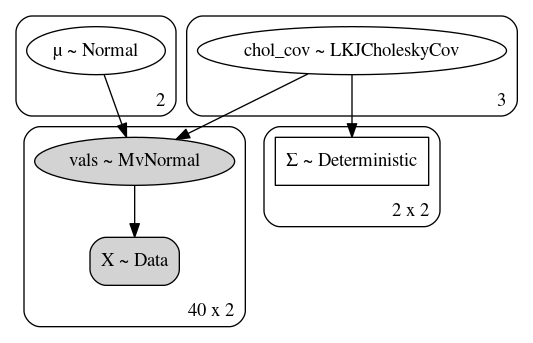
\includegraphics[width=\linewidth]{img/gen/pp_mvn_graph.png}
	\caption{Граф байесовской модели для оценки параметров многомерного нормального распределения}
	\label{fig:pp_mvn_graph}
\end{figure}

\begin{figure}[h!]
	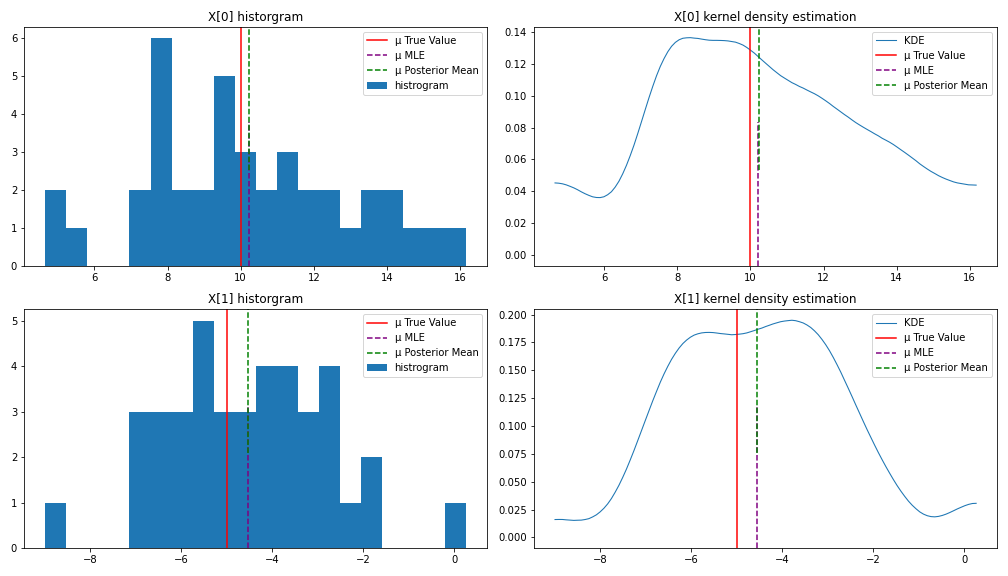
\includegraphics[width=\linewidth]{img/gen/pp_mvn_mu_comparison.png}
	\caption{Сравнения гистограммы данных с оценками $\mu$ (KDE -- Kernal Density Estimation, метод локальной аппроксимации плотности)}
	\label{fig:pp_mvn_mu_comparison}
\end{figure}


\begin{figure}[h!]
	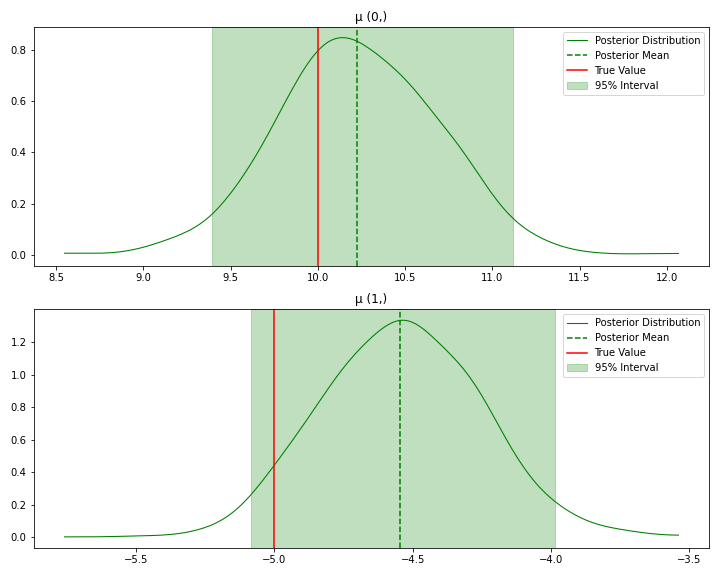
\includegraphics[width=\linewidth]{img/gen/pp_mvn_mu_hdi.png}
	\caption{Сравнение апостериорной оценки $\mu$ с настоящим значением}
	\label{fig:pp_mvn_mu_hdi}
\end{figure}


\begin{figure}[h!]
	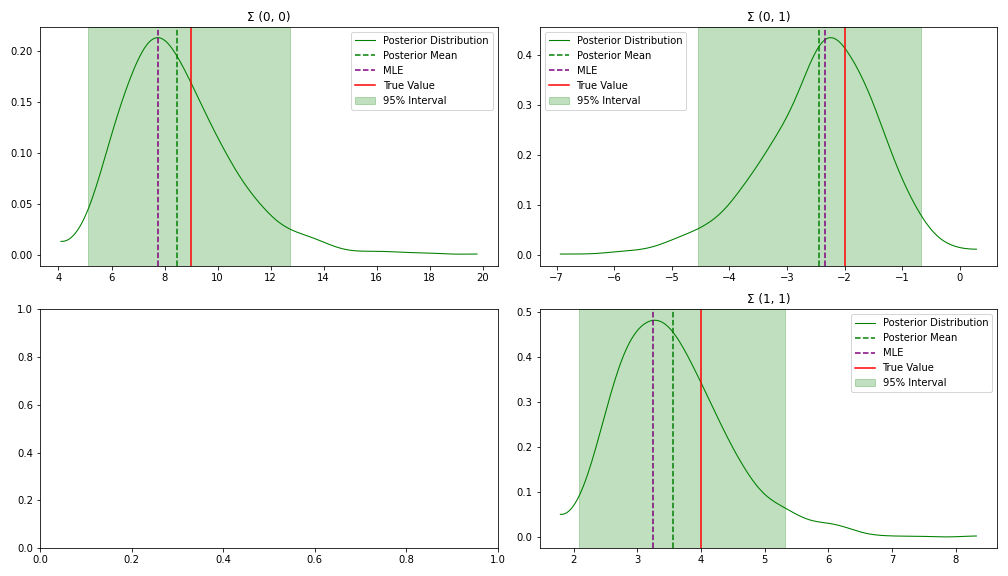
\includegraphics[width=\linewidth]{img/gen/pp_mvn_sigma_hdi.png}
	\caption{Сравнение апостериорной оценки $\Sigma$ с настоящим значением}
	\label{fig:pp_mvn_sigma_hdi}
\end{figure}

На рисунке \ref{fig:pp_mvn_mu_comparison} отображены гистограммы и оценки плотности значений наблюдений $\mathbf{X}$, истинное значение параметра, а также оценки значений методом максимального правдоподобия (MLE) и апостериорного среднего (posterior mean). Как видно, для неинформативных априорных значений эти оценки совпадают. На рисунке \ref{fig:pp_mvn_mu_hdi} отображены апостериорные распределения средних значений и 95\%-е интервалы по сравнению с истинным значением. Для матрицы ковариации можно такие же оценки рассмотреть на рисунке \ref{fig:pp_mvn_sigma_hdi}; видно, что совпадают оценки максимального правдоподобия и максимум апостериори, а среднее апостериорного распределения смещено.


\subsection{VAR model?}

TODO: Add this?


\subsection{RS-Poisson model?}

TODO: Add this? Based on work by \cite{blog_hidden_markov_ravinutala}.


\subsection{RS-MLR model?}

TODO: Add this?


\chapter{Применение MS-VARX к задаче оценки поворотных точек бизнес-цикла экономики Республики Беларусь}

% TODO: Описать данные, метод экспертных оценок, метод фильтрации (кратко, уже была ссылка)


\section{Описание исходных данных}

Как было описано в первой части данной работы, RS-модели могут применяться к задаче определения фаз бизнес-цикла. В качестве базового индикатора бизнес-цикла рассматривается реальный ВВП (GDP) Республики Беларусь в ценах 2014 г. в месячном исчислении; он же рассматривается в качестве моделируемой переменной. Вышеописанный Индекс Экономических Настроений (ESI) используется в качестве экзогенной переменной. Так как ESI является опережающим индикатором (поворотные точки ESI опережают поворотных точек GDP на 2-4 месяца \cite{esiMaking,esiExtra}), рассматриваются варианты моделей со включением различных лагов этой переменной (опережение рассматривалось от 0 до 5 периодов).


\section{Исследование рядов GGDP, GESI статистическими тестами}

Для тестирования интегрированности рядов GGDP и GESI (и их первых разностей) использовались тесты, допускающие наличие структурных изменений. Используя тест BPUR (Breakpoint Unit Root), гипотеза об интегрированности с <<инновационными аномалиями>> (сдвигами) не была отклонена. С помощью теста Баи – Перрона (Bai – Perron tests for sequentially determined breaks) и построении моделей со структурными изменениями (Breakpoint Least Squares) выявлен феномен <<кобрейкинга>> (одновременного структурного изменения) рядов GGDP и GESI. Более подробно процедура описана в \cite{mak_mal_bv_2020}, где также построены две ARX модели (формулы 4 и 5 в статье), не включающие изменения в параметрах т. к.  структурные изменения в GGDP и GESI совпадают. Также было проведено тестирование на коинтегрированность этих рядов, в котором гипотеза о коинтеграции не отклонилась \cite{mak_mal_bv_2020}. 

Принятая методология определения фаз бизнес-цикла экономики Республики Беларусь предполагает две фазы (<<спад>> и <<подъем>>), поэтому фиксируется количество классов $L=2$ которые интерпретируются соответствующим образом. В данной работе везде использовался класс моделей MS-ARX вследствие предыдущих работ автора и руководителя по данной тематике \cite{mak_mal_bv_2018,malVARforCycles}.

Цель экспериментальной части \cite{mak_mal_bv_2020} состоит в оценивании предиктивных способностей моделей MS-ARX, включающие вышеописанный опережающий индикатор. Ряды GDP, ESI содержат сезонные эффекты. В представляемых моделях использовались годовые темпы ростов этих рядов GGDP и GESI соответственно, которые можно рассматривать как сезонно скорректированные ряды. Их циклические компоненты демонстрируют опережающий характер GESI\_C по отношению к GGDP\_C \cite{mak_mal_bv_2020}, см. [PICTURE].


\section{Эксперименты с MS-ARX и опережающим индикатором}

При моделировании GGDP рассматривались некоторые модели семейства MS-ARX, включающие различные структурные предположения и экзогенные переменные. Везде рассматривалось $L=2$ класса и порядок авторегрессии не более $p=2$, т. е. класс MS(2)-ARX(2). В дальнейших формулах используются обозначения $y_t = \text{GGDP}_t$, $x_t = \text{GESI}_t$, и $\eta_t$ -- инновационный процесс.

Из рассмотренных моделей, следующие сошлись и дали лучшие результаты:

\begin{equation}
	M.0. \quad y_t = c_{l(t)} + \alpha_{l(t), 1} y_{t-1} + \alpha_{l(t), 2} y_{t-2} + \eta_t
\end{equation}

Модель $M.0$ не содержит экзогенных факторов и предполагает, что циклические изменения обусловлены аномалиями в инновационном процессе $\eta$ и ведут к изменениям среднего уровня GGDP.

Для моделей $M.1$ - $M.3$ отключено изменение в авторегрессионных коэффициентах $\alpha_i$; вследствие незначимости этих коэффициентов, они исключены в итоговых вариантах моделей.
% TODO: Проверить правильно ли это – может просто не включали изначально?

\begin{equation}	
	M.1. \quad y_t = c_{l(t)} + \alpha_1 y_{t-1} + \alpha_2 y_{t-2} + \beta_{l(t), 1} t + \eta_t
\end{equation}

Модель $M.1$ допускает циклические изменения в трендовой компоненте. 

В основе $M.2$ лежит долгосрочная коинтеграционная зависимость между GGDP и GESI, включающая линейный тренд:

\begin{equation}
	M.2. \quad y_t = c_{l(t)} + \alpha_1 y_{t-1} + \alpha_2 y_{t-2} + \beta_{l(t), 1} t + \beta_{l(t), 2} x_{t} + \eta_t
\end{equation}

$M.3$ включает такую же структуру, однако включает опережающую экзогенную переменную GESI(-4):

\begin{equation}
	M.3. \quad y_t = c_{l(t)} + \alpha_1 y_{t-1} + \alpha_2 y_{t-2} + \beta_{l(t), 1} t + \beta_{l(t), 2} x_{t-4} + \eta_t
\end{equation}

Все коэффициенты при экзогенных переменных зависят от класса состояния $l_t$.

В таблицах [TABLE] и [TABLE] приведены характеристики оцененных моделей, включая коэффициенты, интерпретацию фаз <<роста>> и <<падения>>, и вероятности переходов. На основании этих данных можно сделать следующие выводы:

\begin{enumerate}
	\item Свободный член и включенные в модели экзогенные переменные действительно подвержены циклическим изменениям во всех моделях.
	\item В моделях $M.0$, $M.1$, $M.2$ в состоянии <<спад>> GGDP чувствительна к изменениям в свободном члене и всех включенных переменных (тренд, GESI, авторегрессионная часть), а в состоянии <<рост>> влияет только свободный член.
	\item В модели $M.3$ с опережающей переменной GESI(-4) все коэффициенты значимые, и сама модель обладает наилучшей предиктивной способности при определении двух классов состоянии.
\end{enumerate}


\begin{figure}[h!]
	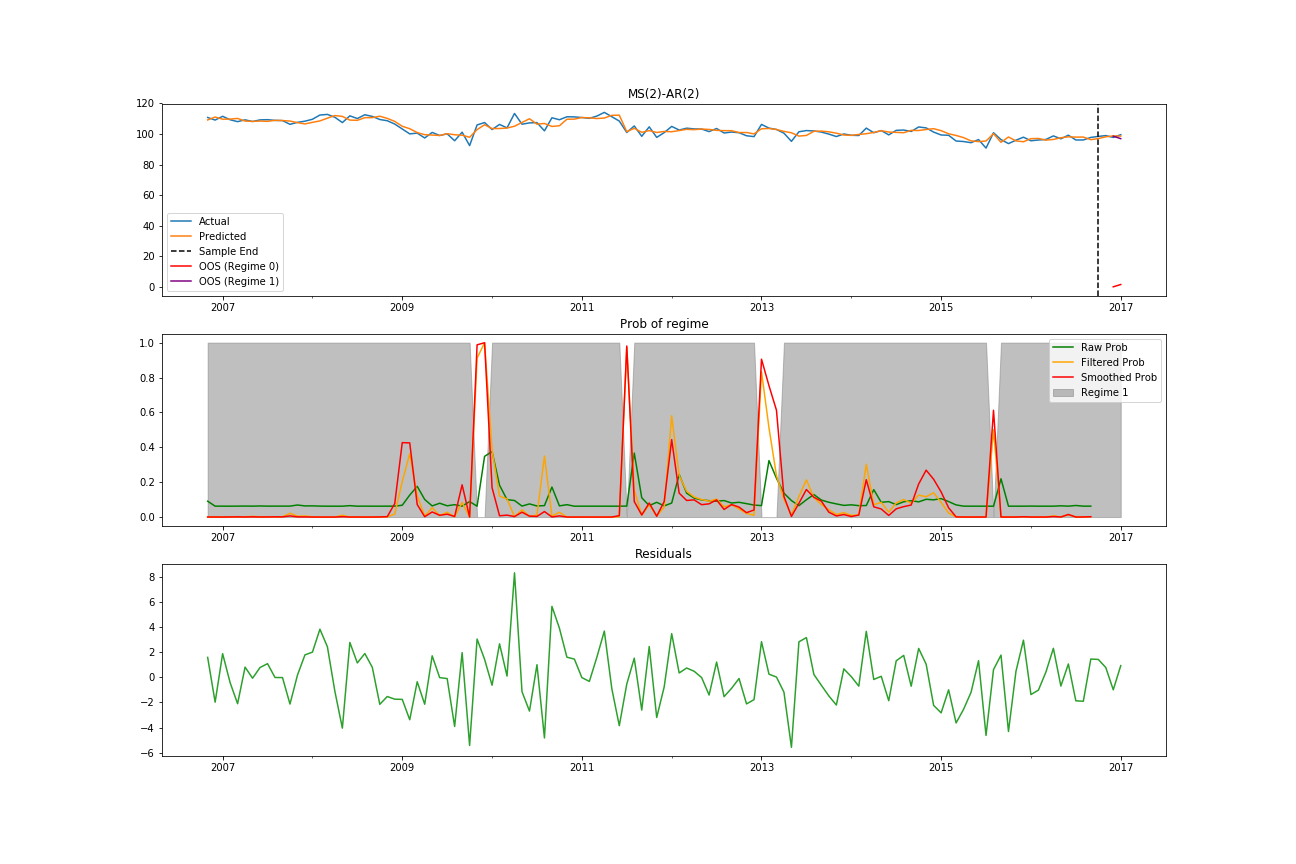
\includegraphics[width=\linewidth]{img/manual/model_m0.png}
	\caption{Модель $M.0$}
	\label{fig:sm_model_m0}
\end{figure}


Графическое представление результатов экспериментов дано на рисунках \ref{fig:sm_model_m0} [PICTURES]. На них представлены:


\begin{itemize}
	\item динамика годовых темпов роста реально ВВП (GGDP),
	\item интервалы соответствующие классам <<роста>> и <<спада>>,
	\item прогнозы моделей для периода оценивания,
	\item условные прогнозы моделей вне этого периода (для валидации).
\end{itemize}

% TODO: Рассказать о сглаженных и несглаженных вероятностях.


% Заключение (выводы)
\fakechapter{Заключение}

TODO: Conclusion.


% Список использованных источников
% \fakechapter{Список использованных источников}
\printbibliography[title=Список использованных источников]
\addcontentsline{toc}{chapter}{Список использованных источников}
\markboth{Список использованных источников}{Список использованных источников}

% Графический материал

% Программы (при необходимости)

% Приложения (при необходимости)


\end{document}